	\begin{figure}[t]
		\centering
		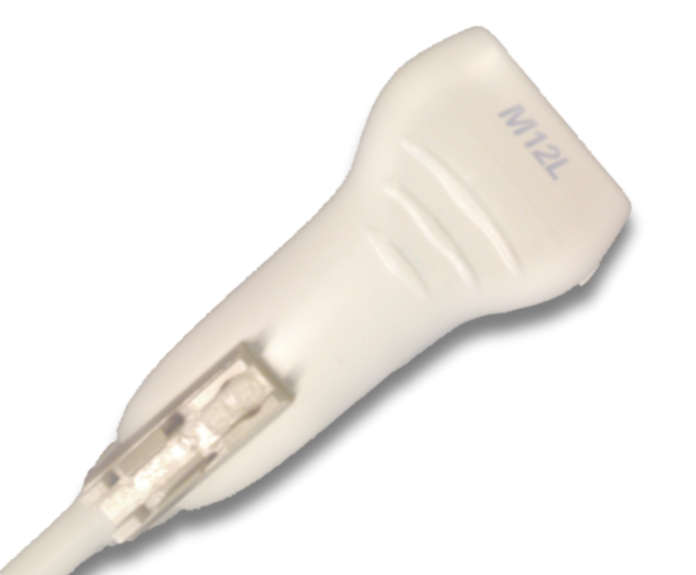
\includegraphics[height=0.3\textheight]{graphics/ultrasound_probe.png}
		\caption[Ultrasound probe]{GE M12L linear array ultrasound probe (GE Healthcare, Waukesha, Wisconsin, USA)}
		\label{fig:ultrasound_probe}
	\end{figure}

In medicine, ultrasound probes such as the one shown in Figure \ref{fig:ultrasound_probe} are used to obtain 2D ultrasound scans called \emph{b-scans}. The probe both emits ultrasound pulses and detects their echo returned. See Figure \ref{fig:ultrasound_principle} for an illustration. As the ultrasound pulse travels through tissue, echoes are created when it encounters materials with varying density. Some of the pulse energy is absorbed by the tissue, some is reflected back as echo and some continues to move forward.
	
	\begin{figure}[b]
		\centering
		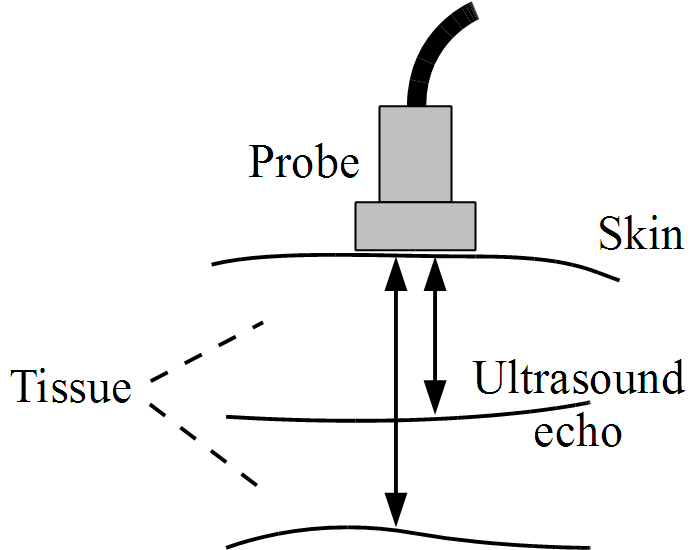
\includegraphics[height=0.25\textheight]{graphics/ultrasound_principle.png}
		\caption{The basic principles of ultrasound in medicine}
		\label{fig:ultrasound_principle}
	\end{figure}

The speed of sound depends on the transmission material, but one can assume a constant speed of $v_{sound} = 1540$ $m/s$ in human tissue \cite{anderson2000}. It should be noted that in reality the speed varies depending on the material, and can be as low as $1450$ $m/s$ in fat and over $1600$ $m/s$ in muscle, but we do not take this into consideration. This means that the distance $d$ from the transducer to the density variation can be estimated by the time $t$ it took for the echo to arrive at the transducer:

	\begin{equation}
		d = \frac{tv_{sound}}{2}
		\label{eq:ultrasound_distance}
	\end{equation}
	
The strength of the echo is given by the difference between acoustic impedances of the materials next to each other. If the probe emits and receives ultrasound in a linear array, a 2D image can be formed where the height is the distance from the probe, the width is the width of the array and the intensity of a pixel is the strength of the echo. The resulting image is the ultrasound b-scan. The array can also be curved, giving a \emph{curvilinear} b-scan. Examples of linear and curvilinear b-scans are shown in Figure \ref{fig:b-scan_examples}.

	\begin{figure}[h]
	\centering
	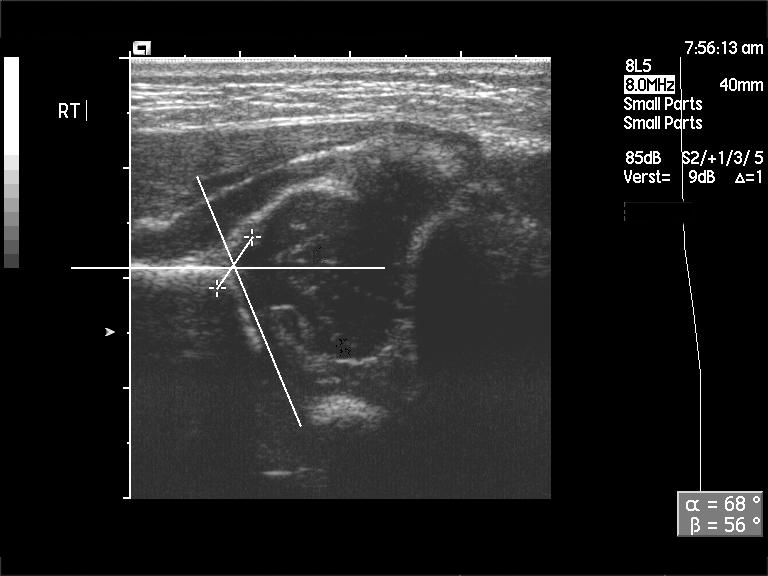
\includegraphics[width=0.49\textwidth]{graphics/linear_b-scan.png}
	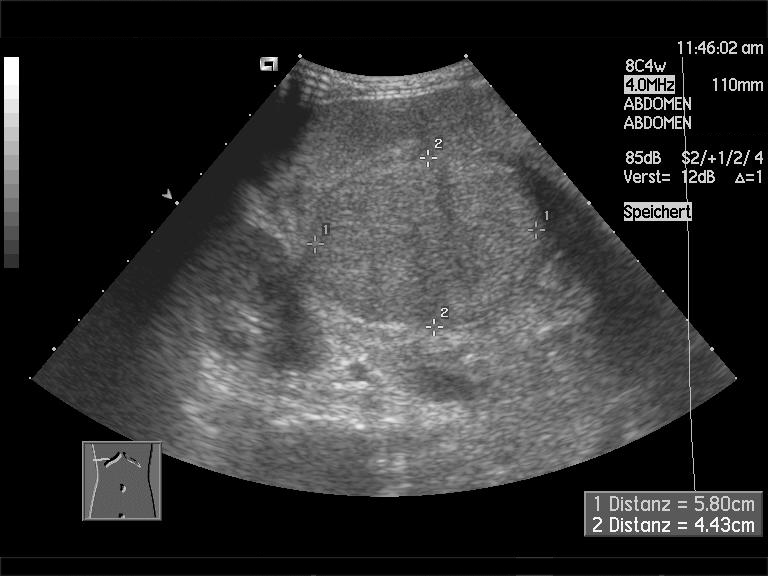
\includegraphics[width=0.49\textwidth]{graphics/curvilinear_b-scan.png}
	\caption[Linear and curvilinear b-scans]{Linear and curvilinear b-scans (used with permission from A. Christaras)}
	\label{fig:b-scan_examples}
	\end{figure}

To construct a 3D volume, each b-scan is tagged with a timestamp and location and rotation of the probe in 3D space. This data together with the b-scans is then processed, which can take minutes to hours depending on the desired quality of the reconstructed output. Once reconstructed, the volume can be used for many purposes. Typically, it can be visualized using direct volume rendering through ray casting or similar methods. But other techniques are also used, such as multiplanar reformatting slices (MPR slices) that are created from the volume. The MPR slices are planar slices of sampled points through the volume, like cutting it in half with a sharp flat knife. More details about visualization of 3D ultrasound data is found in Section \ref{section:ultrasound_visualization}, and description of how to reconstruct a volume from b-scans is found in Section \ref{section:ultrasound_reconstruction}.